\chapter{Two Sides of a Battlefield: Japanese Cemetery and Commonwealth War Cemetery}

\section{Two Cemeteries, One Island}

Singapore is an extraordinarily small island, yet within this tiny space it holds buried, side by side, the two sides of a single war.

On one side is the Japanese Cemetery Park --- silent in a corner of the city, overgrown weeds tangled with bougainvillea, headstones weathered, time-worn and mottled. On the other is Kranji War Memorial Park, maintained and funded by the Commonwealth War Graves Commission, with manicured lawns and rows of white headstones standing in solemn, orderly lines.

The former holds the aggressors, and the women history has forgotten. The latter holds the invaded, and the memory of a city's fall.

\section{Japanese Cemetery Park: A Place Forgotten by Time}

The Japanese Cemetery Park is located in the northeastern part of Singapore, in Hougang, at 22 Chuan Hoe Ave. Covering approximately 29,000 square meters and containing 910 headstones, it is the largest Japanese cemetery in Southeast Asia. In 1969, the Singapore government transferred ownership of the cemetery to the \textbf{Japanese Association of Singapore}, which has been responsible for its day-to-day maintenance ever since; in 1987, the site was formally designated a memorial park.

Walking into the Japanese Cemetery Park, the first sensation is quiet.

Not the solemn quiet of formal reverence, but the quiet of something forgotten. Most of the headstones in the cemetery are low and plain, surfaces covered in moss; some have tilted, some have crumbled. Bright magenta bougainvillea climbs in from the sides, draping itself over several of the stones --- blooms vivid and brilliant against the grey, forming a strange contrast. Life and death, juxtaposed here in a way you wouldn't expect.

\begin{figure}[h]
\centering
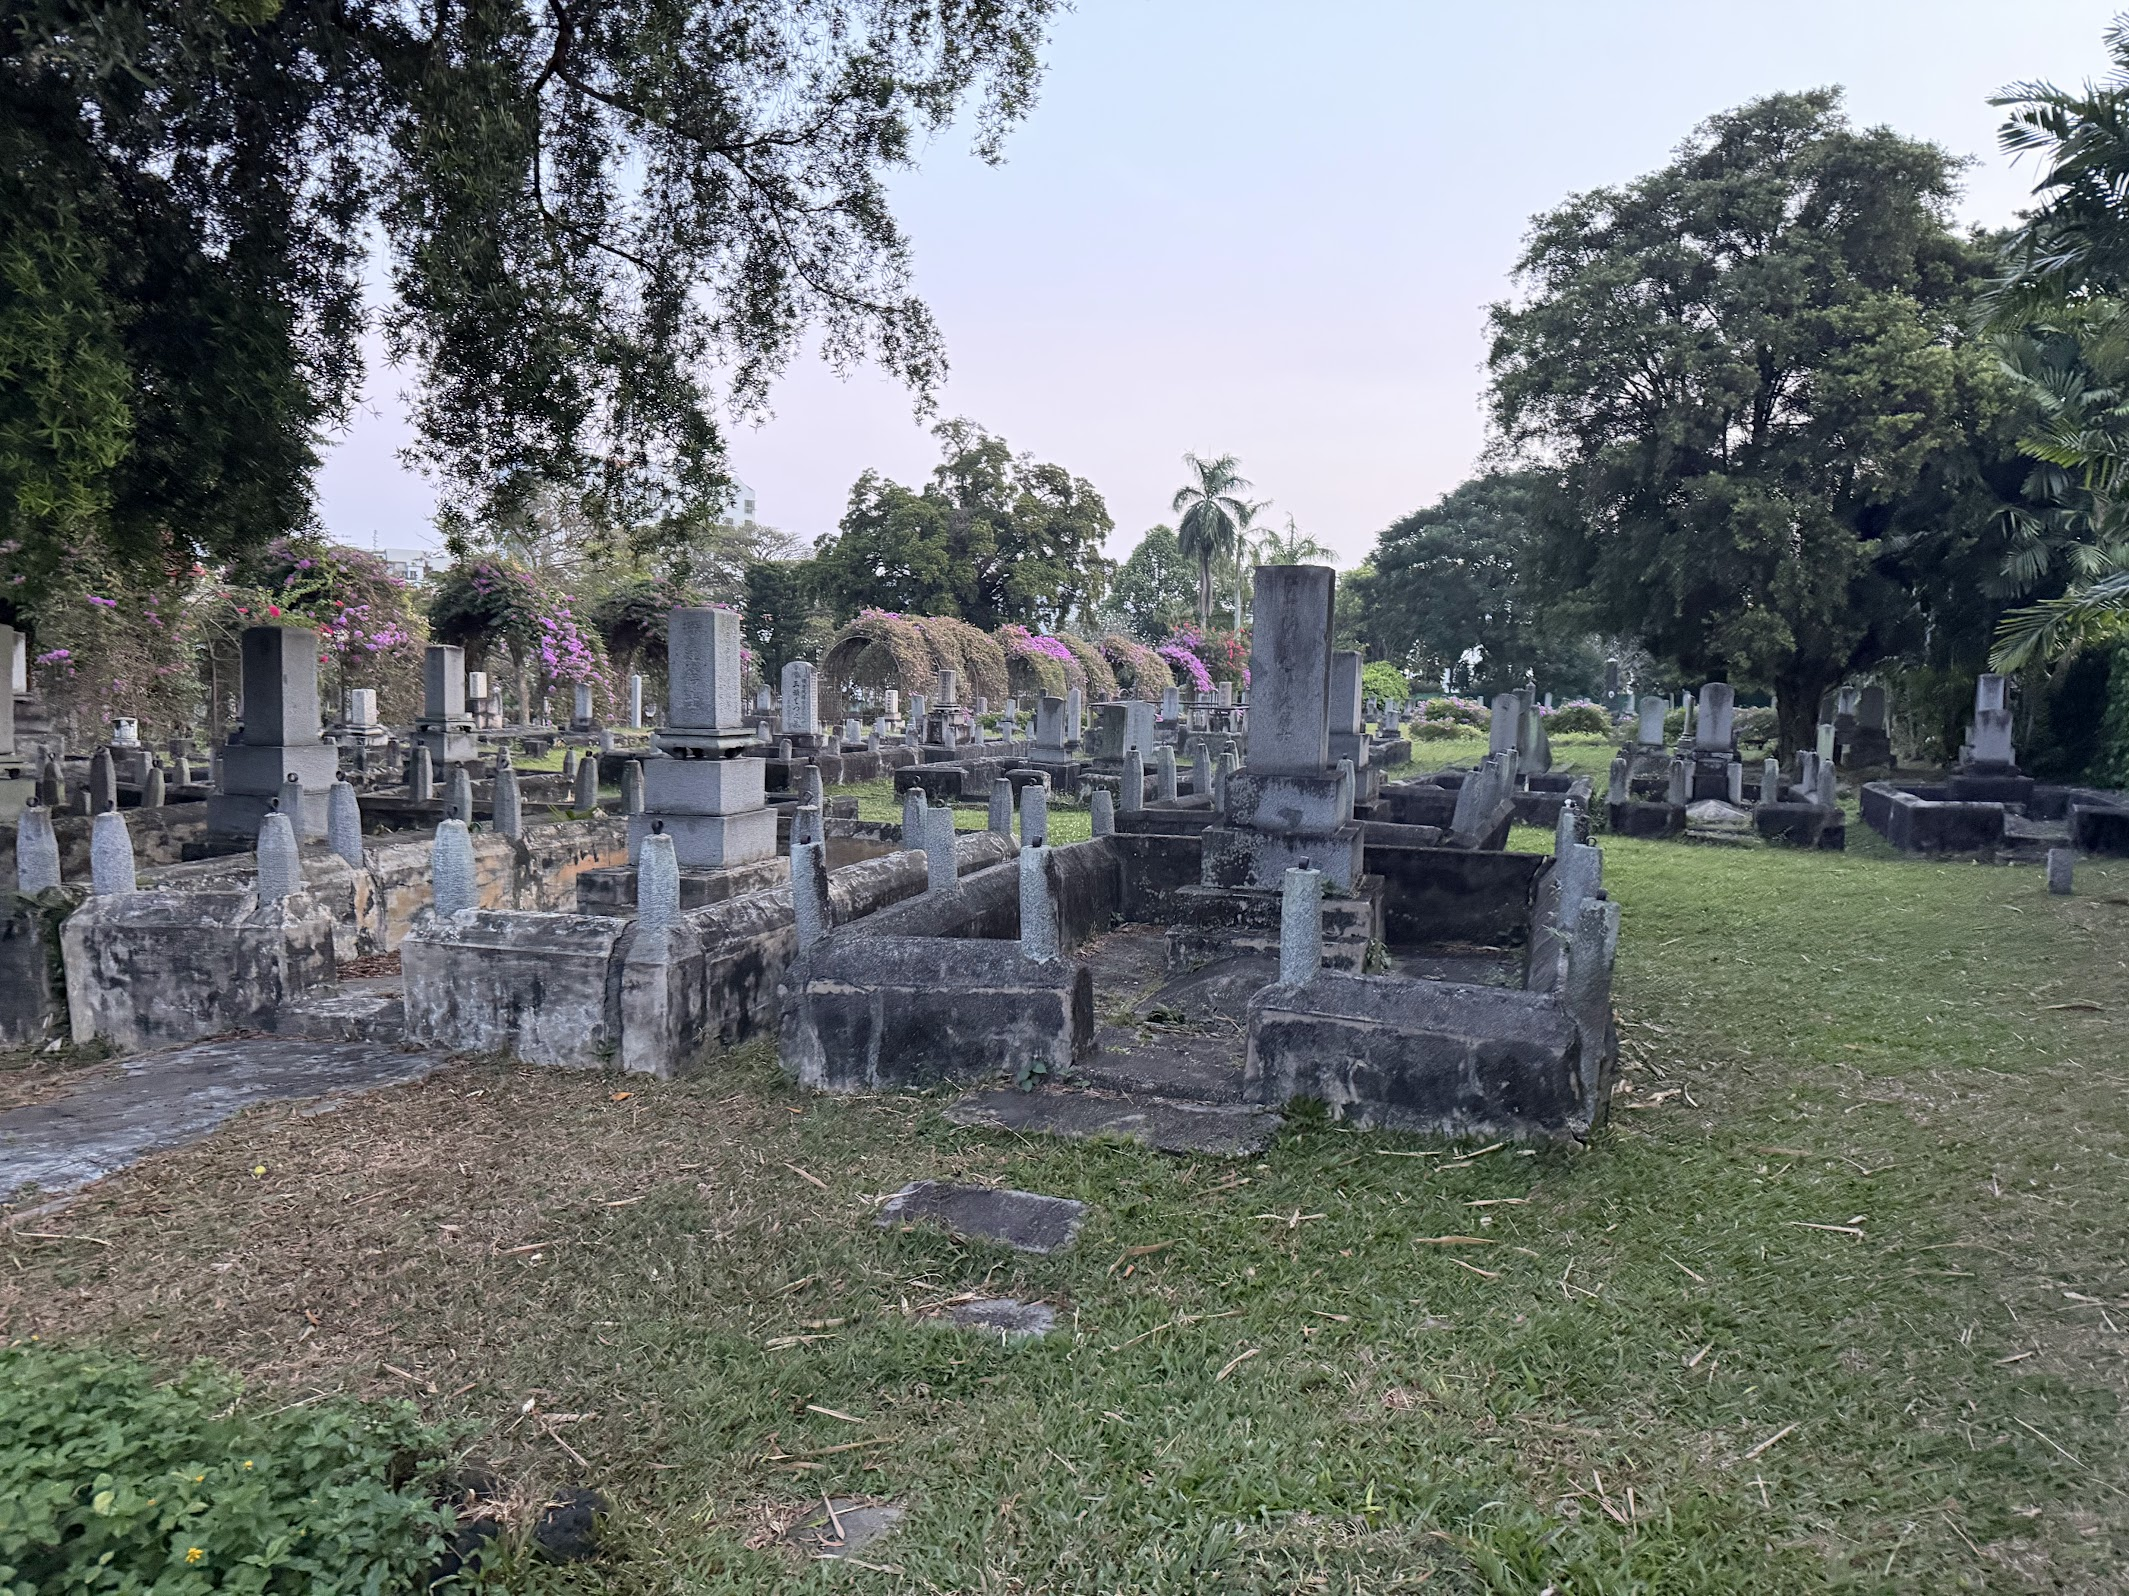
\includegraphics[width=0.8\textwidth]{../../pictures/japanese tomb/IMG_9019}
\caption{Bougainvillea climbing over a weathered headstone}
\end{figure}

Across the open grass, dozens of headstones are scattered at uneven intervals, arranged with no deliberate order. In the soft light of morning or evening, the entire cemetery feels especially empty.

\begin{figure}[h]
\centering
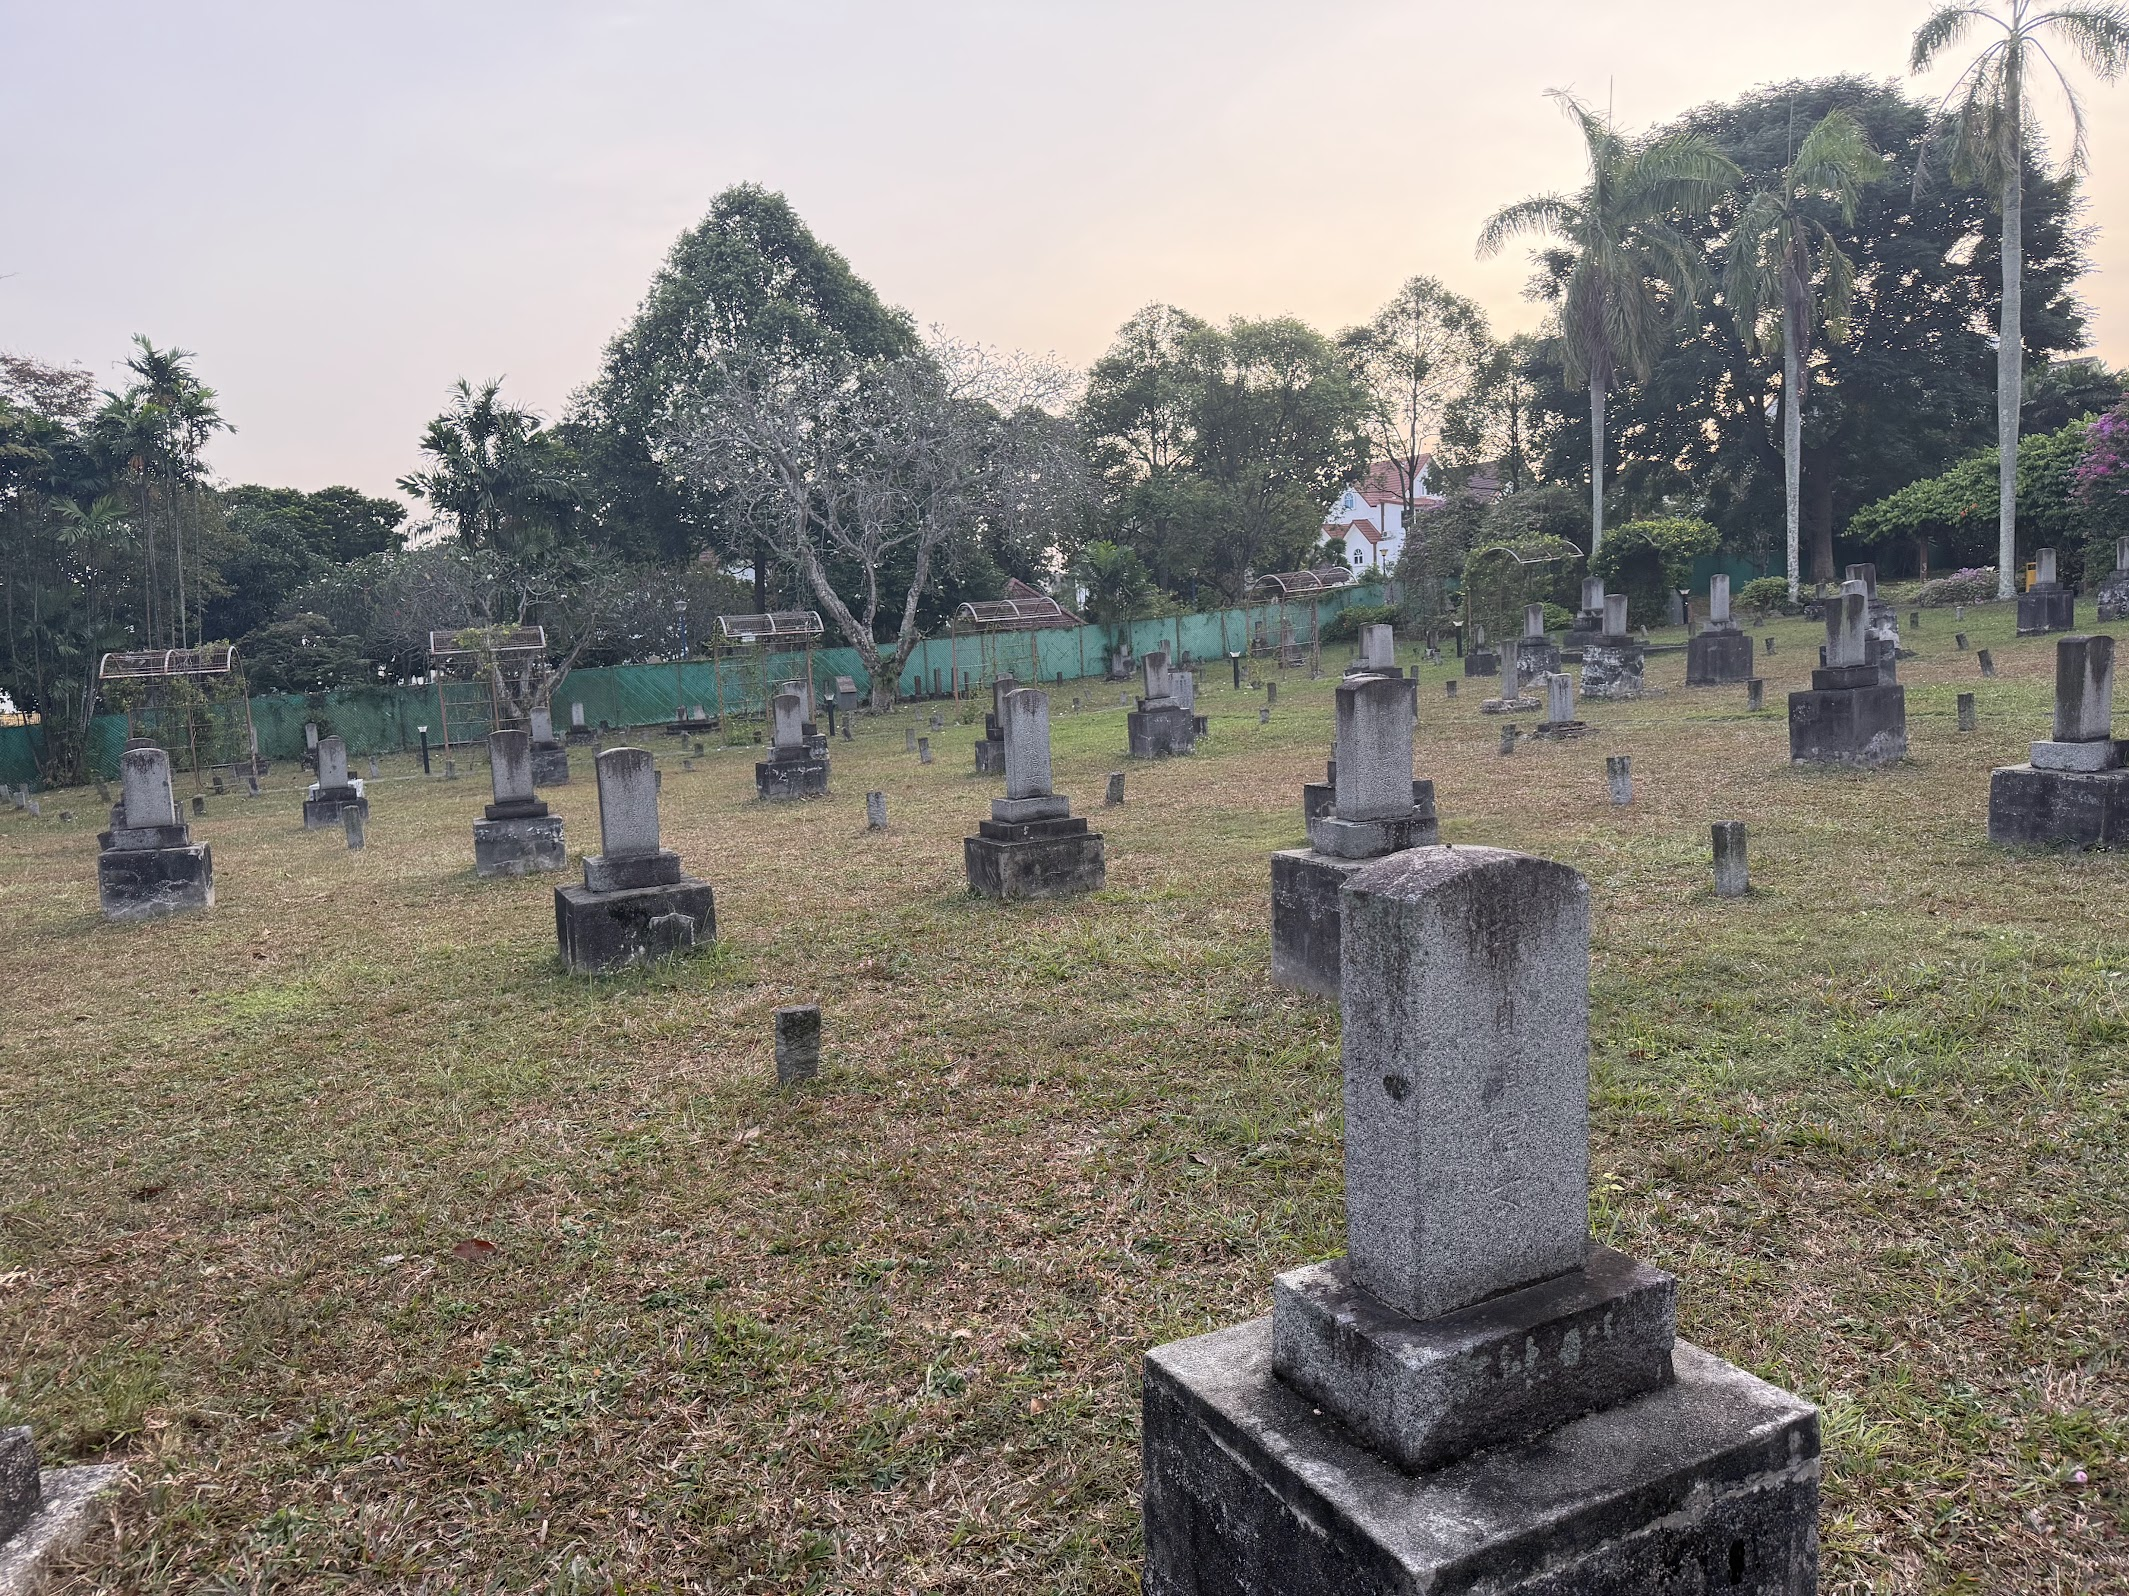
\includegraphics[width=0.8\textwidth]{../../pictures/japanese tomb/IMG_9080}
\caption{Panoramic view: low headstones scattered across the grass}
\end{figure}

\section{Pioneer Cemetery: Seventy-Seven Named Women}

In one corner of the cemetery stands a sign, its heading reading ``\begin{CJK}{UTF8}{min}先進墓地\end{CJK}'' --- Pioneer Cemetery.

The sign introduces a woman named \textbf{Toma Sato}, who died in 1899. She was a \textbf{karayuki-san} --- from the late nineteenth to early twentieth century, large numbers of Japanese women traveled overseas to Southeast Asia, many of whom worked in the sex trade. They were called ``karayuki-san,'' meaning ``those who went to Tang-land (China),'' though in practice they traveled throughout all of Southeast Asia.

The sign records that within this walled enclosure are \textbf{77 graves}, all belonging to karayuki-san, with dates of death ranging from \textbf{1899 to 1938}. This plot of land was once used by the British colonial government as a boundary marker --- even in death, their bodies became coordinates on a colonial map.

\begin{figure}[h]
\centering
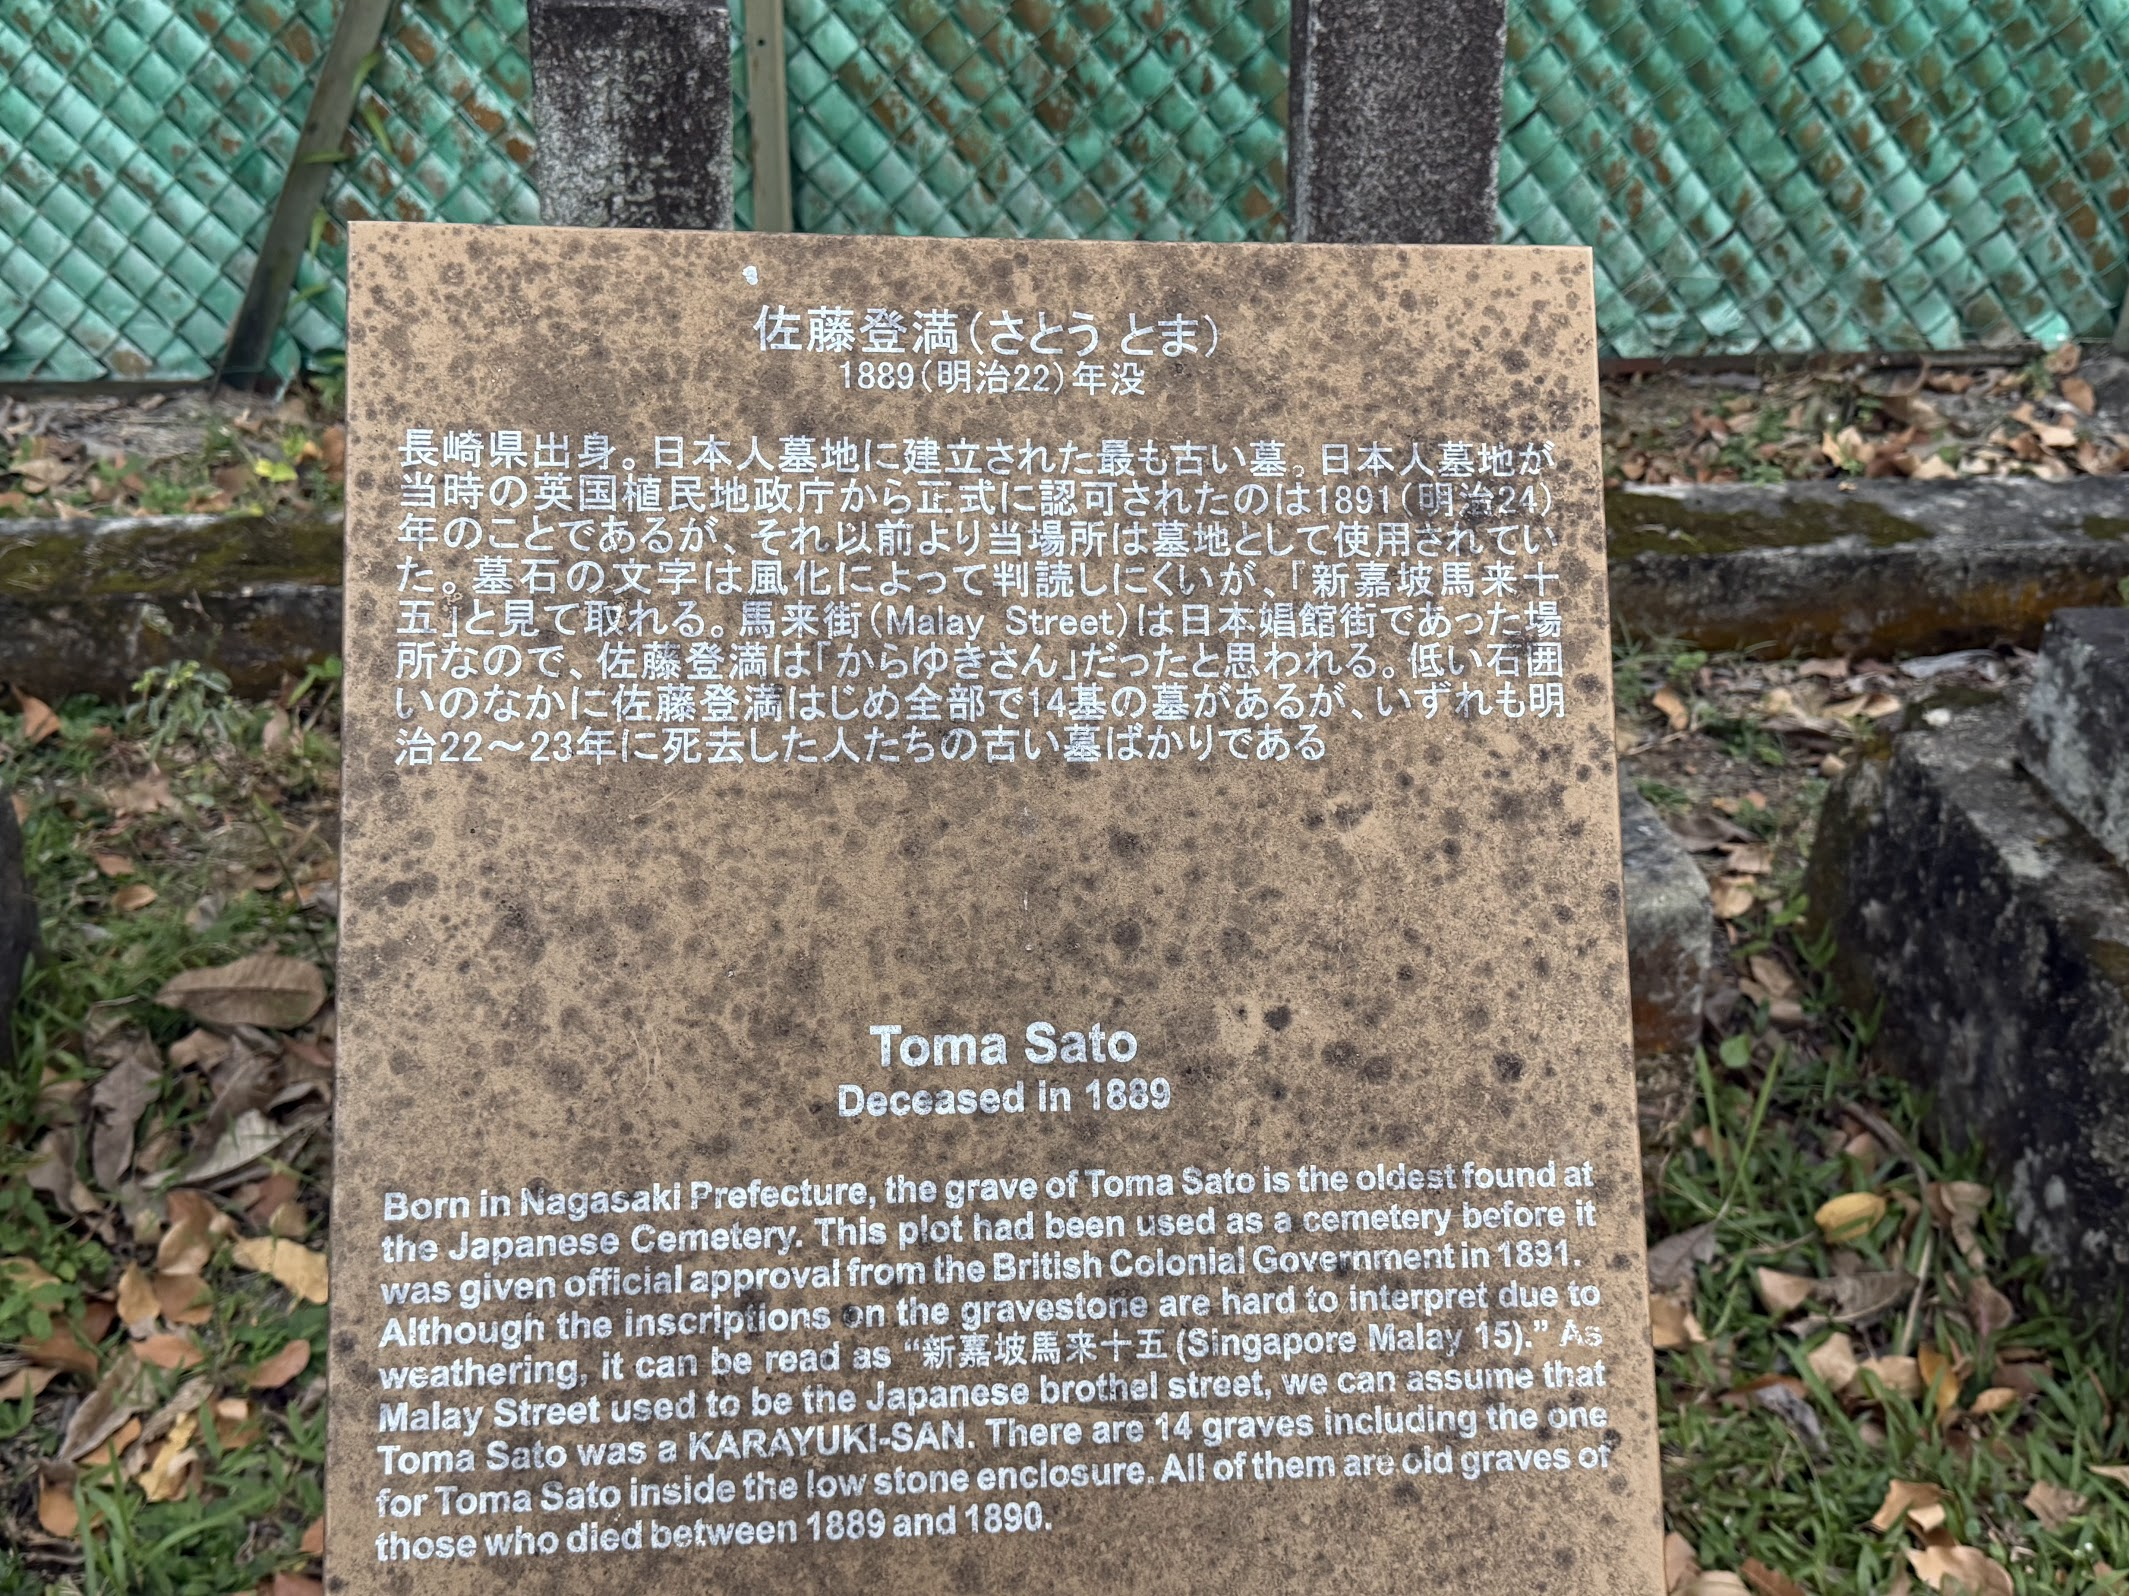
\includegraphics[width=0.8\textwidth]{../../pictures/japanese tomb/IMG_9048}
\caption{Pioneer Cemetery sign introducing Toma Sato and the 77 karayuki-san}
\end{figure}

The Singapore government has placed this sign here in Chinese, English, and Japanese, formally acknowledging ``KARAYUKI-SAN'' --- and that acknowledgment is itself a form of historical recognition. Yet what comes after recognition?

\section{Someone Still Remembers}

Elsewhere in the cemetery, a relatively well-preserved Japanese stone tablet stands alone. Its face is carved with Japanese characters, and before it sit an incense burner and an offering table. The ash is fresh --- someone was here not long ago.

In this cemetery where most have been forgotten, this one stone stands out as something precious. Someone remembers. Perhaps a descendant, perhaps someone quietly guarding this piece of history.

\begin{figure}[h]
\centering
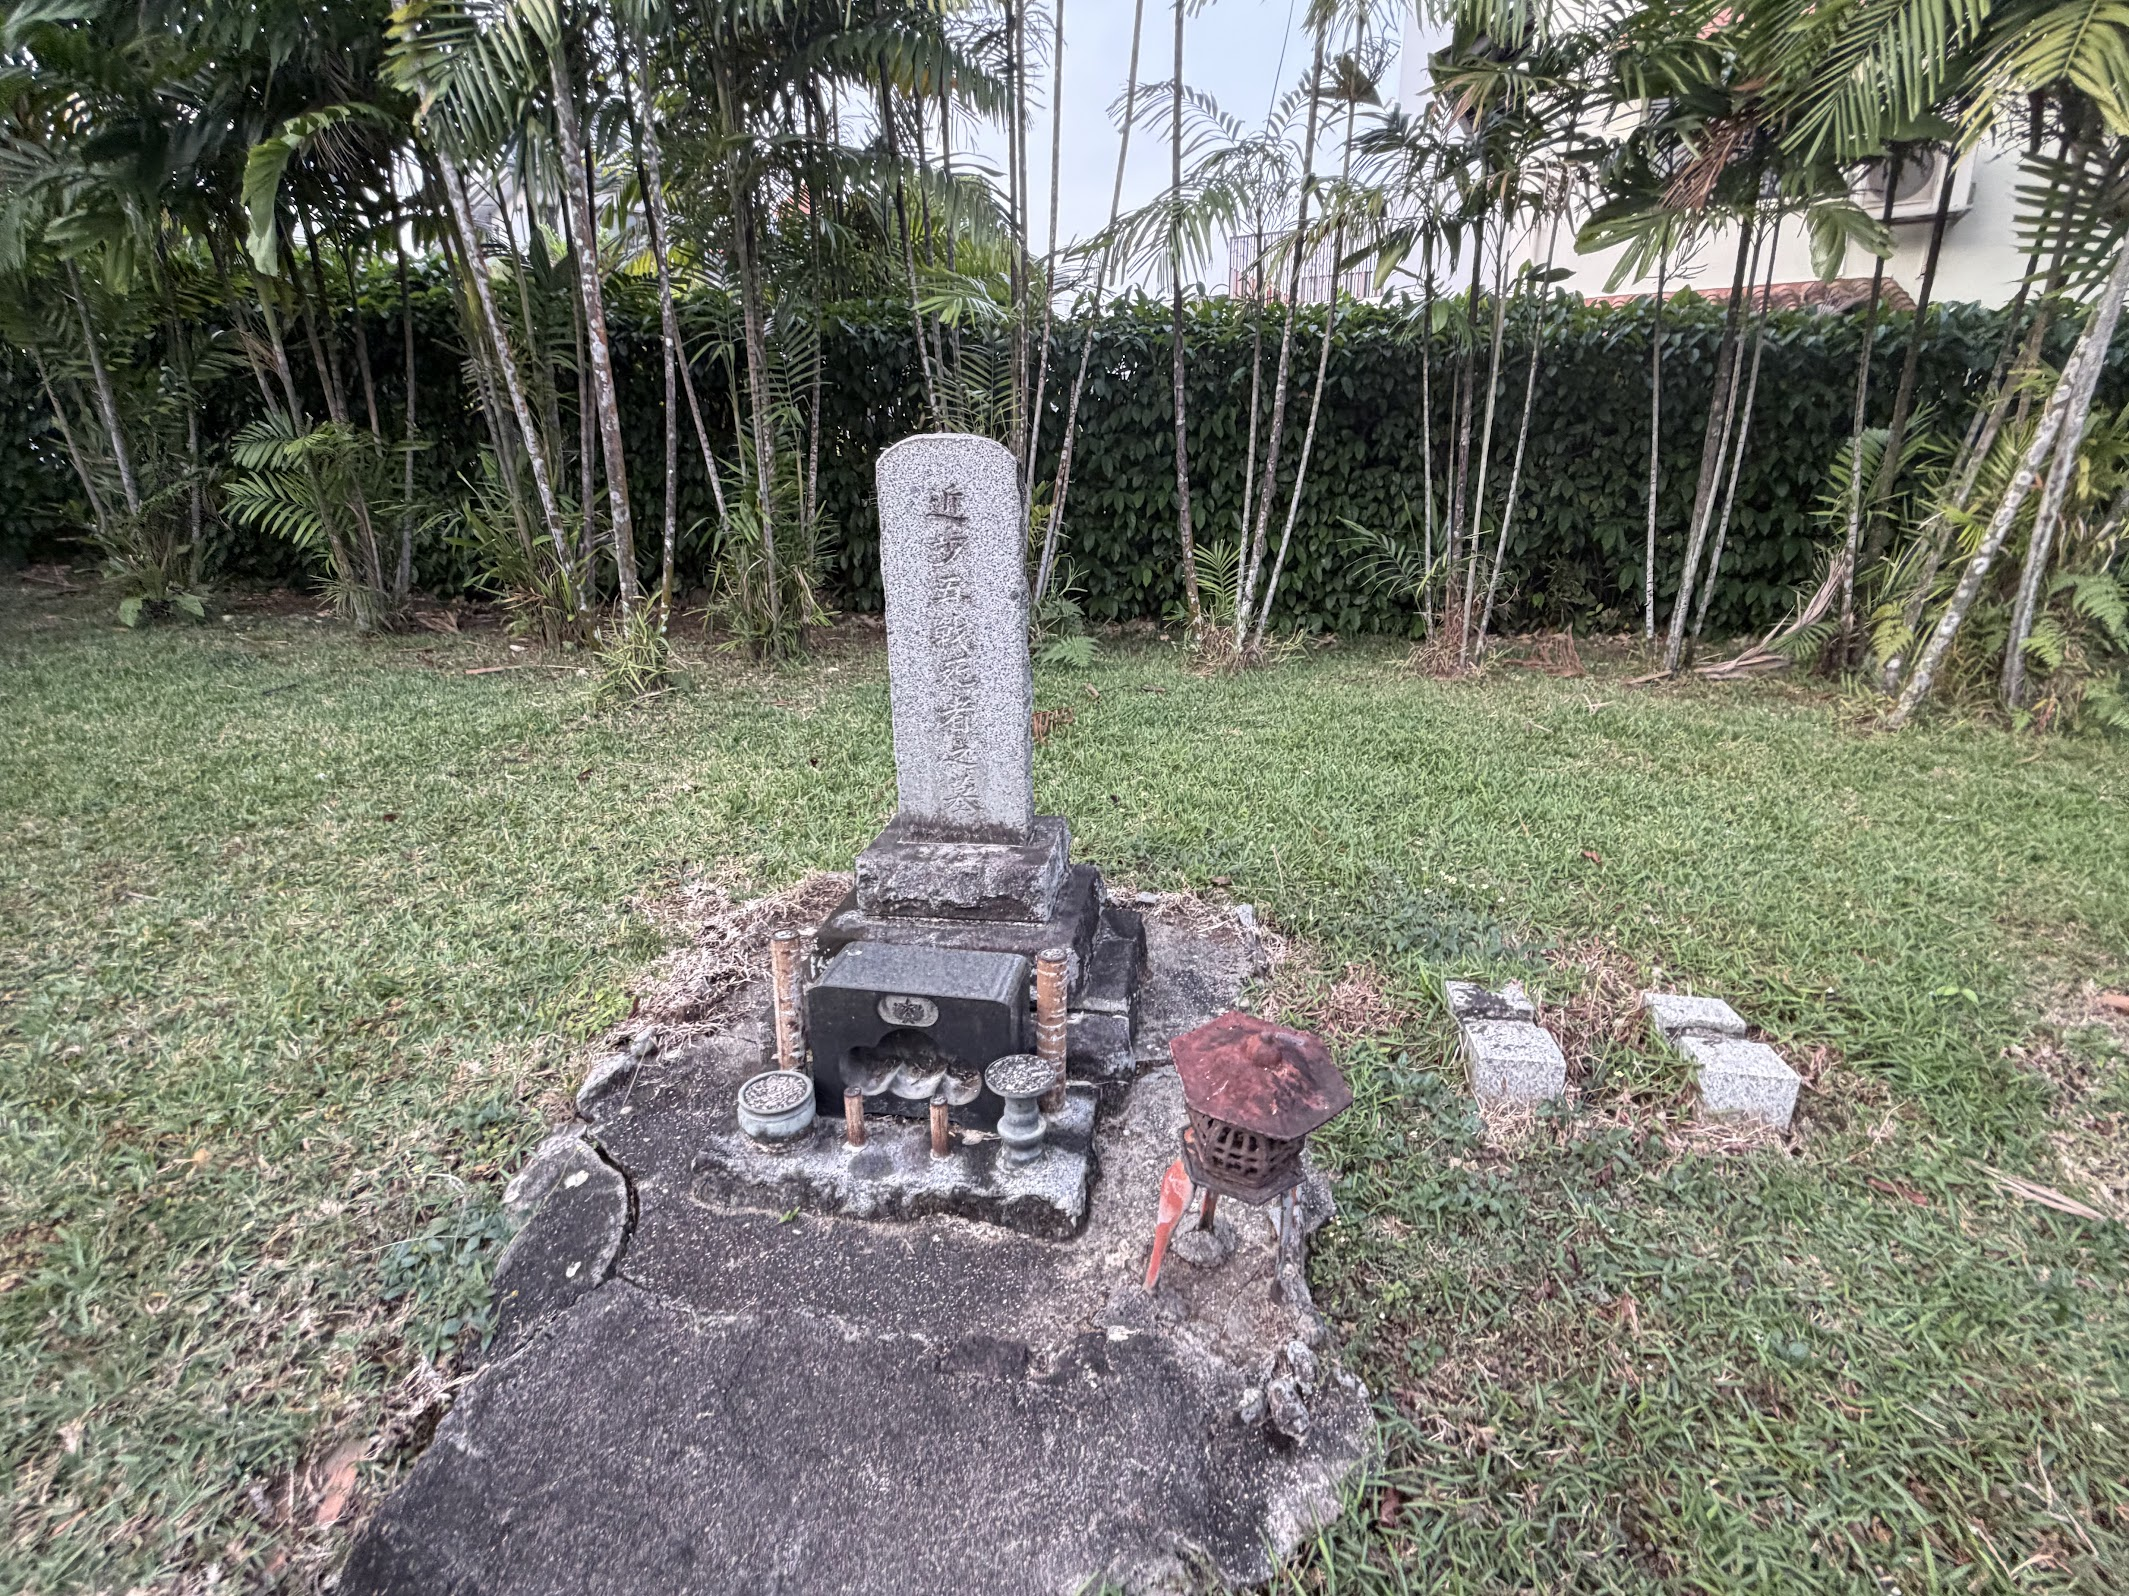
\includegraphics[width=0.8\textwidth]{../../pictures/japanese tomb/IMG_9124}
\caption{A headstone still tended, with incense burner and offerings}
\end{figure}

On the other side of the cemetery, stone benches are arranged along a winding stone path. The atmosphere here is no longer entirely that of a cemetery --- it feels more like a park. Singapore's positioning of this land is dual: a place of remembrance, and a public green space for residents to rest.

\begin{figure}[h]
\centering
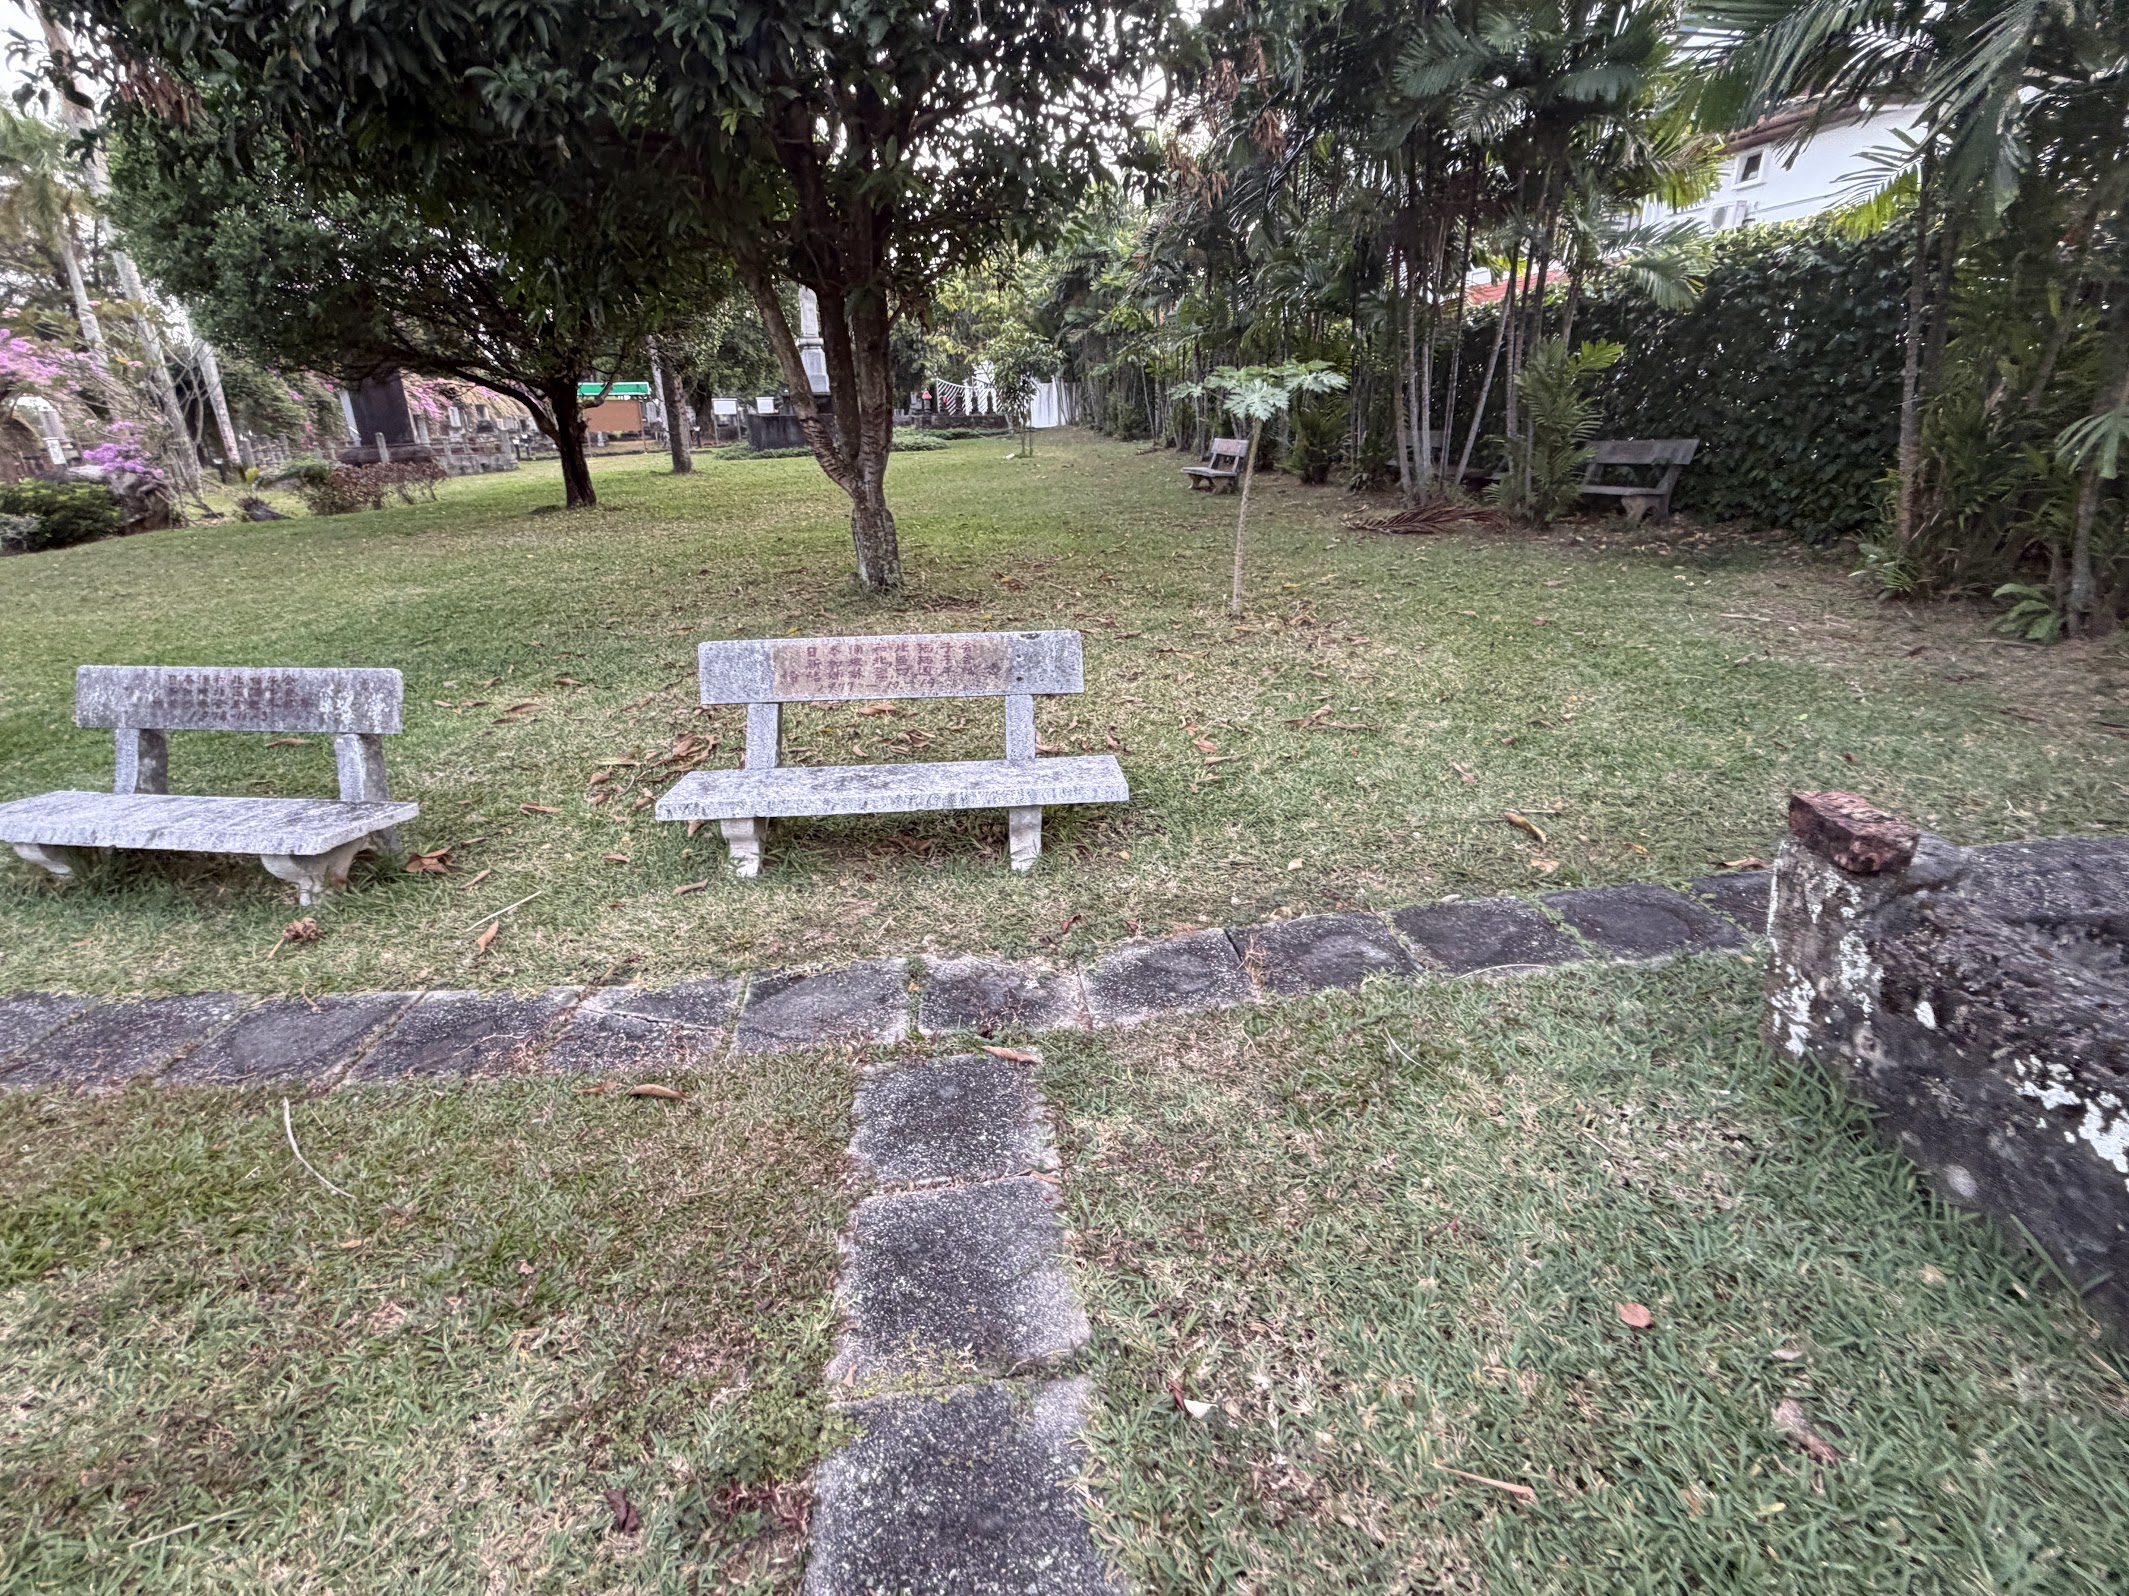
\includegraphics[width=0.8\textwidth]{../../pictures/japanese tomb/IMG_9129}
\caption{Stone benches and winding path --- atmosphere more like a park}
\end{figure}

This duality invites contemplation. Is the parkification of this space a form of inclusion --- or a gentle forgetting?

\section{Kranji: A Different Way of Remembering}

Compared to the overgrown quietude of the Japanese Cemetery Park, Kranji War Memorial Park is another world entirely.

Kranji War Cemetery is located in northern Singapore, at 9 Woodlands Road, set on high ground along the northern shore of Singapore Island, overlooking the Straits of Johore across the water toward Malaysia. This location is no accident --- on February 8, 1942, it was precisely across this strait that the Japanese forces crossed, landing near the mouth of the Kranji River, less than three kilometers from where the cemetery stands today.

Leading that assault was General Tomoyuki Yamashita, commander of the Japanese 25th Army. Before attacking Singapore, his forces had already swept southward down the Malay Peninsula --- using bicycles instead of horses, pedaling through jungle and road, covering the distance from southern Thailand to the northern shore of Singapore in roughly 70 days. This ``Bicycle Blitzkrieg'' caught the British forces completely off guard, and Yamashita earned the nickname the \textbf{``Tiger of Malaya.''} The British heavy guns had been pointed south toward the open sea, guarding against an enemy expected to come from the water --- they never imagined the enemy would arrive from behind, on bicycles.

The cemetery is maintained by the Commonwealth War Graves Commission (CWGC), and kept in perpetually immaculate condition. White headstones stand in neat rows on precisely trimmed lawns, solemn and restrained. Buried here are Allied soldiers who fell during the Fall of Singapore in 1942 --- servicemen from Britain, Australia, India, Malaya, and elsewhere who gave their lives resisting the Japanese advance.

Every headstone is carved with a name, rank, and date. There are no unknown graves.

This way of remembering is organized, funded, and institutionally guaranteed. The memory of the victors tends to be more lasting --- and more orderly --- than the memory of the defeated.

\section{Who Is Remembered, Who Is Forgotten}

Standing between these two cemeteries, I kept turning over the same question: who is remembered, and who is forgotten?

The soldiers at Kranji have names, have nations, have a commission to weed and tend their graves and maintain their records. The 77 karayuki-san in the Japanese cemetery were, for most of history, almost entirely unknown --- until a single sign appeared, and allowed their existence to be seen by those who passed by.

They were not warriors. They were not heroes. Even in their own country they were figures shrouded in shame. Yet they too died on this island, and they too were received by its tropical earth.

Singapore today enjoys friendly relations with Japan, with close economic ties. This wartime history has neither been loudly prosecuted nor completely erased. The Japanese cemetery still stands; the sign still stands. This may be Singapore's way of handling history: preserve, but do not amplify; acknowledge, but do not become entangled.

A small nation surviving on the blade's edge has little margin left for hatred.
